\documentclass[style=sailor,size=12pt]{powerdot}
\usepackage{epic,array,ecltree,url,calrsfs}
\usepackage[nointegrals]{wasysym}
\usepackage{listings}
\usepackage{epsfig}
\usepackage{amsmath}
\usepackage{amsfonts}
\usepackage{amssymb}
\usepackage{amsxtra}
\usepackage{amsthm}
\usepackage{mlextra} % Must be below ams packages
\usepackage{mathrsfs}
\usepackage{color}
\usepackage{array}
\usepackage{graphicx}
\graphicspath{ {../art/} }
\usepackage{bm}
\usepackage{tikz}
\usepackage{multicol}
\usepackage{enumitem}

\newcommand{\treenode}{%
  \begingroup\normalfont
  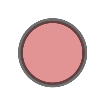
\includegraphics[height=\fontcharht\font`\c]{node.eps}%
  \endgroup
}

\newcommand{\tripletreenode}{%
  \begingroup\normalfont
  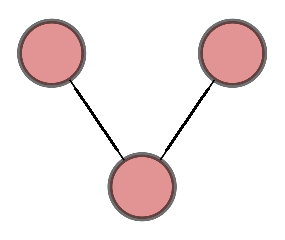
\includegraphics[height=\fontcharht\font`\B]{3nodetree.eps}%
  \endgroup
}

\pdsetup{method=normal}

\title{Systems and Proof: Part I}
\author{Foundations of Computer Science}
\date{\today}

\begin{document}
\maketitle
\begin{slide}[toc=,bm=]{Overview}
This slide set covers the following topics:

\vspace{5mm}
\tableofcontents[content=sections]
\end{slide}

\section[slide=true]{Expressing Recursive Definitions with Post Systems} 
\include{sap_content/sap_post}

\section[slide=true]{Proof by Strong Induction}
\begin{wideslide}[bm=,toc=]{Strong induction}
\begin{itemize}
\item A Post system supposedly for positive multiples of 3:
\vspace{-1em}
\begin{tabbing}
{\bf R2}XX \=  \kill
{\bf B} \>
        \(\begin{array}[t]{l}
        3\in S
        \end{array}\) \\[2ex]
{\bf R} \>
        \(\begin{array}[t]{l}
        x \in S \;\;\;y \in S \\
        \hline
        x + y \in S
        \end{array}\)
\end{tabbing}
\item We shall prove the soundness and completeness of this system with respect to
the set of all positive multiples of 3.
\end{itemize}
\end{wideslide}

\begin{wideslide}[bm=,toc=]{Soundness by strong induction}
{\bf Theorem}. $n\in S$ iff $n$ is a positive multiple of 3.
\vspace{1em}

{\bf Proof}.  As the statement is an ``iff'', it has two parts, the ``only-if'' part (soundness)
and the ``if'' part (completeness).

\vspace{1em} 
(only-if): $n\in S$ only if $n$ is a positive multiple of 3.

\vspace{1em} 
(if): if $n$ is a positive multiple of 3 then $n\in S$. 
\end{wideslide}


\begin{wideslide}[bm=,toc=]{Soundness by strong induction}
(only-if): $n\in S$ only if $n$ is a positive multiple of 3.
This is proved by strong induction on the height of the derivation of $n\in S$.

\vspace{1em}
$S(k)$: if the derivation of $n\in S$ has height $k$ then $n$ is a positive multiple of 3.

\begin{displaymath}
\begin{array}[t]{l}
S(0) \\
\forall k\geq 0.\, S(0)\wedge \cdots \wedge S(k)\Rightarrow S(k+1) \\
\hline
\forall k\geq 0.\, S(k)
\end{array}
\end{displaymath}

\vspace{1em}
Basis: Show $S(0)$.

\vspace{1em}
Inductive hypothesis: Suppose $S(0),\ldots ,S(k)$ {\bf where} $k\geq 0$.

\vspace{1em}
Inductive step: Show $S(k+1)$.
\end{wideslide}

\begin{wideslide}[bm=,toc=]{Soundness: basis and inductive step}
{\em $S(0)$\/}: derivation height is zero. \\ 
Then the derivation must end with an
application of rule {\bf B}, which implies $n=3$.
And 3 is a positive multiple of 3 since $3\cdot 1=3$.

\vspace{1em}
{\em $S(k + 1)$}.
We must show $n$ is a positive multiple of 3 if $n\in S$ has derivation height $k+1$ and $k\geq 0$.

\vspace{1em}
Suppose $n\in S$ has derivation height $k+1$ and $k\geq 0$.
Then since $k\geq 0$, the derivation must end with an application of rule {\bf R}.
Thus $n$ can be expressed as the sum of $i$ and $j$ where $i\in S$ and $j\in S$.
By induction, $i$ and $j$ are positive multiples of $3$, meaning there are positive integers
$a$ and $b$ such that $i=3a$ and $j=3b$.
Hence 
\[n = i + j = 3a + 3b = 3(a+b)
\]
thus establishing $n$ is a positive multiple of 3.
\end{wideslide}

\begin{wideslide}[bm=,toc=]{Completeness by weak induction}
(if): if $n$ is a positive multiple of 3 then $n\in S$.
All positive multiples of 3 can be expressed as $3k$ for some positive integer $k$.
We prove by {\em weak induction\/} on $k \in \N$ that $3k\in S$.


\vspace{1em}
$S(k)$: if $k$ is a positive integer such that $k\geq 1$ then $3k\in S$.

\begin{displaymath}
\begin{array}[t]{l}
S(1) \\
\forall k\geq 1.\, S(k)\Rightarrow S(k+1) \\
\hline
\forall k\geq 1.\, S(k)
\end{array}
\end{displaymath}

\vspace{1em}
Basis: Show $S(1)$.

\vspace{1em}
Inductive hypothesis: Suppose $S(k)$ {\bf where} $k\geq 1$.

\vspace{1em} 
Inductive step: Show $S(k+1)$.
\end{wideslide}

\begin{wideslide}[bm=,toc=]{Completeness by weak induction}
{\em $S(1)$\/}: $k=1$.\\  
\vspace{1em}
By axiom {\bf B}, $3\in S$ so $3k\in S$ since $3k = 3$.

\vspace{2em}
{\em $S(k + 1)$}:
We must show $3(k+1)\in S$ where $k\geq 1$.\\
\vspace{1em}
We have $3(k+1) = 3k + 3$.
By induction, $3k\in S$ and by axiom {\bf B}, $3\in S$.
Therefore by rule {\bf R}, $3k + 3\in S$, or $3(k+1)\in S$.
\end{wideslide}

\begin{wideslide}[bm=,toc=]{Strong induction multiple base cases}
\begin{itemize}
\item A Post system with multiple axioms.
\vspace{-1em}
\begin{tabbing}
{\bf R1}XX \=  \kill
{\bf B1} \>
        \(\begin{array}[t]{l}
        4\in P
        \end{array}\) \\[2ex]
{\bf B2} \>
        \(\begin{array}[t]{l}
        5\in P
        \end{array}\) \\[2ex]
        
{\bf R} \>
        \(\begin{array}[t]{l}
        x \in P \;\;\;y \in P \\
        \hline
        x + y \in P
        \end{array}\)
\end{tabbing}
\item Claim: any postage of 12 cents or more can be formed using only 4 and 5-cent stamps (Rosen pg.\ 337).
\item Claim is proven by showing any positive integer at least 12 belongs to {\em P\/}.
\item This is a {\em completeness\/} result of the Post system.
\item We say nothing about soundness of the system because it's not of interest. 
%namely $P=\{4,5,8,10,12,13,14,\ldots\}$.
\end{itemize}
\end{wideslide}

\begin{wideslide}[bm=,toc=]{Completeness by strong induction}
$S(n)$: if $n$ is a positive integer such that $n\geq 12$ then $n\in P$.

\begin{displaymath}
\begin{array}[t]{l}
S(12) \wedge S(13) \wedge S(14) \wedge S(15) \\
\forall n\geq 15.\, S(12)\wedge S(13)\wedge S(14)\wedge S(15)\wedge\cdots\wedge S(n)\Rightarrow S(n+1) \\
\hline
\forall n\geq 12.\, S(n)
\end{array}
\end{displaymath}

\vspace{1em}
Basis: Show $S(12),S(13),S(14)$ and $S(15)$.

\vspace{1em}
Inductive hypothesis: Suppose $S(12), \ldots , S(n)$ {\bf where} $n\geq 15$.

\vspace{1em}
Inductive step: Show $S(n+1)$.
\end{wideslide}

\begin{wideslide}[bm=,toc=]{Completeness by strong induction}
If $n$ is a positive integer such that $n\geq 12$ then $n\in P$.

\vspace{1em}
The proof is by strong induction on $n$.
Suppose $n\geq 12$.

\vspace{1em}
{\em Basis\/}: There are four cases: $n=12$, $n=13$, $n=14$ and $n=15$.

\vspace{1em}
$12\in P$ by 3 applications of rule {\bf B1} and two applications of {\bf R}.

$13\in P$ by 2 applications of {\bf B1}, one application of {\bf B2} and two applications of {\bf R}.

$14\in P$ by 2 applications of {\bf B2}, one application of {\bf B1} and two applications of {\bf R}.

$15\in P$ by 3 applications of {\bf B2} and two applications of {\bf R}.

\vspace{1em}
{\em Inductive hypothesis\/}:  Suppose $n\geq 15$ and $k\in P$ if $12\leq k \leq n$.

\vspace{1em}
{\em Inductive step}.
We must show $n+1\in P$ where $n\geq 15$.
Since $n\geq 15$, $n+1-4\geq 12$.
By induction, $n-3\in P$.
By axiom {\bf B1}, $4\in P$.
So by rule {\bf R} $n-3+4\in P$ or $n+1\in P$.
\end{wideslide}

%\end{document}
%
%Suppose $t\in\id{RT}$ has derivation height $n+1$ where $n\geq 0$.
%Then the derivation must end with {\bf R2}. 
%Therefore $t$ has the form $\id{node}(x)$
%where $x\in\id{RTL}$.
%The derivation of $x\in\id{RTL}$ has height $n$.
%%So by induction and $S_1$, $\id{\#edges}(x)=\id{\#nodes}(x)$.
%Then
%\begin{displaymath}
%\begin{array}{lll}
%\id{\#nodes}(\id{node}(x)) & = & 1 + \id{\#nodes}(x) \\
%	& = & 1+\id{\#edges}(x) + |x|\;\;\;\rid{by induction and}\;S_1 \\
%	& = & 1+\id{\#edges}(\id{node}(x))
%\end{array}
%\end{displaymath}
%Ergo, $\id{\#edges}(\id{node}(x))=\id{\#nodes}(\id{node}(x))-1$.
%\end{wideslide}
%
%\begin{wideslide}[bm=,toc=]{Mutual induction}
%Now we show $S_1$.
%Suppose $l\in\id{RTL}$ has derivation height $n+1$ where $n\geq 0$.
%Then the derivation must end with {\bf R1}. 
%Therefore $l$ has the form $\id{cons}(x,y)$
%where $x\in\id{RT}$ and $y\in\id{RTL}$.
%Either the derivation of $x\in\id{RT}$ or $y\in\id{RTL}$ has height $n$ while the other 
%has height {\em at most\/} $n$.
%%By induction and $S_2$, $\id{\#edges}(x)=\id{\#nodes}(x)-1$.
%%Also by induction and $S_1$, $\id{\#edges}(y)=\id{\#nodes}(y)$.
%Then
%\begin{displaymath}
%\begin{array}{lll}
%\id{\#edges}(\id{cons}(x,y)) & = & \id{\#edges}(x) + \id{\#edges}(y) \\
%	& = & \id{\#nodes}(x) - 1 + \id{\#edges}(y) \\
% & & \>\>\>\>\>\>\rid{by induction and}\;S_2 \\
%	& = & \id{\#nodes}(x) - 1 + \id{\#nodes}(y) - |y| \\
% & & \>\>\>\>\>\>\rid{by induction and}\;S_1 \\
%	& = & \id{\#nodes}(\id{cons}(x,y)) - 1 - |y| \\
%	& = & \id{\#nodes}(\id{cons}(x,y)) - (1 + |y|) \\
%	& = & \id{\#nodes}(\id{cons}(x,y)) - |\id{cons}(x,y)|
%\end{array}
%\end{displaymath}
%%{\em quod erat demonstrandum (Q.E.D.)\/}
%\end{wideslide}


\section[slide=true]{Proof by Mutual Induction}
\begin{wideslide}[bm=,toc=]{Recursive definitions}
\begin{itemize}
\item A mutually-recursive definition of {\em rooted trees\/} {\em RT\/}:
\begin{tabbing}
{\bf R2}XX \=  \kill
{\bf B} \>
        \(\begin{array}[t]{l}
        \id{nil}\in\id{RTL}
        \end{array}\) \\[2ex]
{\bf R1} \>
        \(\begin{array}[t]{l}
        t\in\id{RT}\;\;\;l\in\id{RTL} \\
        \hline
        \id{cons}(t,l)\in\id{RTL}
        \end{array}\) \\[2ex]
{\bf R2} \>
        \(\begin{array}[t]{l}
        l\in\id{RTL} \\
        \hline
        \id{node}(l)\in\id{RT}
        \end{array}\)
\end{tabbing}
\item Compare with definition in Rosen 7th Ed.
\item Rosen ignores mutual recursion and hence mutual induction.
\item His definition is not induction friendly.
\end{itemize}
\end{wideslide}

\begin{wideslide}[bm=,toc=]{Mutual induction}
{\bf Theorem}. If $t\in\id{RT}$ then $\id{\#edges}(t)$ = $\id{\#nodes}(t) - 1$.
\vspace{1em}

{\bf Proof}.  By {\em strong\/} mutual induction on derivation height. 
We prove the following two statements:
\vspace{1em}

$S_1$: $l\in \id{RTL}\Rightarrow \id{\#edges}(l) = \id{\#nodes}(l) - |l|$.

$S_2$: $t\in \id{RT}\Rightarrow \id{\#edges}(t) = \id{\#nodes}(t) - 1$.

\vspace{2em}
Note: $|l|$ stands for the length of list $l$, $\id{\#edges}(l)$ the number of edges in $l$
and $\id{\#nodes}(l)$ the number of nodes in $l$.
\end{wideslide}

\begin{wideslide}[bm=,toc=]{Mutual induction}

\vspace{1em}
$S_1(n)$: if the derivation of $l\in \id{RTL}$ has height $n$ then
$\id{\#edges}(l) = \id{\#nodes}(l) - |l|$.
$S_2(n)$: if the derivation of $t\in \id{RT}$ has height $n$ then
$\id{\#edges}(t) = \id{\#nodes}(t) - 1$.

\vspace{1em}



\begin{displaymath}
\begin{array}[t]{l}
S_1(0)\wedge S_2(0) \\
\forall n\geq 0.\, S_1(0)\wedge S_2(0) \wedge \cdots \wedge
S_1(n)\wedge S_2(n)\Rightarrow S_1(n+1)\wedge S_2(n+1)\\
\hline
\forall n\geq 0.\, S(n)
\end{array}
\end{displaymath}

\vspace{1em}
Basis: Show $S_1(0)$ and $S_2(0)$.

\vspace{1em}
Inductive hypothesis: Suppose $S_1(0), S_2(0), \ldots ,S_1(n),S_2(n)$ {\bf where} $n\geq 0$.

\vspace{1em}
Inductive step: Show $S_1(n+1)$ and $S_2(n+1)$.

\end{wideslide}
\begin{wideslide}[bm=,toc=]{Mutual induction}
{\em Basis\/}: derivation height is zero.

\vspace{1em}
$S_1(0)$: If derivation height is zero then $l\in\id{RTL}$ implies $l=\id{nil}$.
Then $\id{\#edges}(\id{nil})=\id{\#nodes}(\id{nil}) - |\id{nil}| = 0$.

\vspace{1em}
$S_2(0)$: Vacuously true since there's no derivation of height zero for $t\in\id{RT}$.

\vspace{2em}
{\em Inductive hypothesis (restated)\/} :  Suppose for all $k$ where $0\leq k\leq n$ and $n\geq 0$,
$S_1(k)$ holds if $l\in\id{RTL}$ has derivation height $k$ and
$S_2(k)$ holds if $t\in\id{RT}$ has derivation height $k$.
\end{wideslide}

\begin{wideslide}[bm=,toc=]{Mutual induction}
{\em Inductive step}.
We must show $S_1(n+1)$ and $S_2(n+1)$ for $n\geq 0$.
We begin with $S_2(n+1)$.

\vspace{1em}
Suppose $t\in\id{RT}$ has derivation height $n+1$ where $n\geq 0$.
Then the derivation must end with {\bf R2}. 
Therefore $t$ has the form $\id{node}(l)$
where $l\in\id{RTL}$.
The derivation of $l\in\id{RTL}$ has height $n$.
%So by induction and $S_1$, $\id{\#edges}(x)=\id{\#nodes}(x)$.
Then
\begin{displaymath}
\begin{array}{lll}
\id{\#nodes}(\id{node}(l)) & = & 1 + \id{\#nodes}(l) \\
	& = & 1+\id{\#edges}(l) + |l|\;\;\;\rid{by induction and}\;S_1 \\
	& = & 1+\id{\#edges}(\id{node}(l))
\end{array}
\end{displaymath}
Ergo, $\id{\#edges}(\id{node}(l))=\id{\#nodes}(\id{node}(l))-1$.
\end{wideslide}

\begin{wideslide}[bm=,toc=]{Mutual induction}
Now we show $S_1(n+1)$.
Suppose $l'\in\id{RTL}$ has derivation height $n+1$ where $n\geq 0$.
Then the derivation must end with {\bf R1}. 
Therefore $l'$ has the form $\id{cons}(t,l)$
where $t\in\id{RT}$ and $l\in\id{RTL}$.
Either the derivation of $t\in\id{RT}$ or $l\in\id{RTL}$ has height $n$ while the other 
has height {\em at most\/} $n$.
%By induction and $S_2$, $\id{\#edges}(x)=\id{\#nodes}(x)-1$.
%Also by induction and $S_1$, $\id{\#edges}(y)=\id{\#nodes}(y)$.
Then
\begin{displaymath}
\begin{array}{lll}
\id{\#edges}(\id{cons}(t,l)) & = & \id{\#edges}(t) + \id{\#edges}(l) \\
	& = & \id{\#nodes}(t) - 1 + \id{\#edges}(l) \\
 & & \>\>\>\>\>\>\rid{by induction and}\;S_2 \\
	& = & \id{\#nodes}(t) - 1 + \id{\#nodes}(l) - |l| \\
 & & \>\>\>\>\>\>\rid{by induction and}\;S_1 \\
	& = & \id{\#nodes}(\id{cons}(t,l)) - 1 - |l| \\
	& = & \id{\#nodes}(\id{cons}(t,l)) - (1 + |l|) \\
	& = & \id{\#nodes}(\id{cons}(t,l)) - |\id{cons}(t,l)|\\
	& = & \id{\#nodes}(l') - |l'|
\end{array}
\end{displaymath}
%{\em quod erat demonstrandum (Q.E.D.)\/}
\end{wideslide}



\end{document}

